\parindent=0em
\section{Mapbox para búsqueda de rutas}
\label{mapboxbusquedarutas}
\noindent

Como se tratado en el punto~\ref{mapboxpunto}, Mapbox ofrece distintas funciones. En el caso de la búsqueda de rutas se utiliza la función \textit{Navigation}. Esta función aporta de forma muy detallada información sobre las rutas, es por ello y por su facilidad de uso (no requiere facturación) por lo que se ha elegido este servicio para realizar las siguientes pruebas.\\

La función \textit{Navigation}\footnotemark~ ofrece distintas APIs:

\begin{itemize}
    \item \textbf{\textit{Mapbox Directions API}}: Permite calcular rutas óptimas conduciendo, andando y en bicicleta teniendo en cuenta el tráfico, además aporta instrucciones de voz paso a paso. 
    \item \textbf{\textit{Mapbox Matrix API}}: Esta API es utilizada para calcular el tiempo de viaje entre puntos. Se genera una matriz con las distancias entre todos los puntos dados y se escoge la distancia o la duración de trayecto más cortos entre puntos.
    \item \textbf{\textit{Mapbox Optimization API}}: Aporta la posibilidad de obtener una optimización de la duración de una ruta dadas unas coordenadas.
    \item \textbf{\textit{Mapbox Map Macthing API}}: Con esta API se generan los caminos que se van a visualizar en el mapa.
\end{itemize}

\footnotetext{\textit{Nagivation} de Mapbox: \href{https://docs.mapbox.com/api/navigation/}{\nolinkurl{https://docs.mapbox.com/api/navigation/}}}

En este caso la API que es interesante es \textit{Mapbox Directions API}. Se utiliza para obtener la información de ruta entre dos puntos. Cuando esta API recibe dos puntos A y B para crear una ruta entre ellos, disecciona la ruta en partes más pequeñas de cara a ser utilizadas en el navegador por voz. Gracias a esa disección se puede obtener distancias estimadas entre esas partes más pequeñas y hacia que lado hay que girar al llegar a dichas partes para alcanzar el siguiente punto.\\

Esto se puede observar más detalladamente en la figura~\ref{fig:mapboxprogressroute} donde se puede ver la información que aporta Mapbox sobre una ruta. Esta información se puede dividir en tres partes.


\begin{figure}[H]
    \centering
    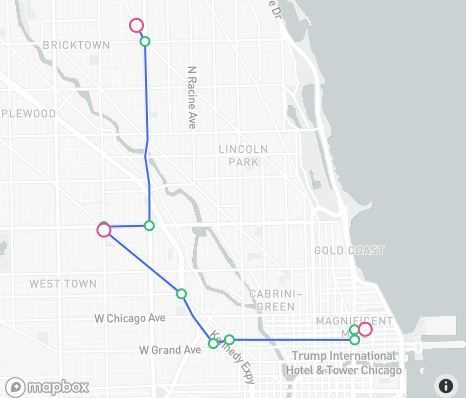
\includegraphics[scale=0.9]{Images/Mapas/mapboxrouteprogress.JPG}
    \caption[Información sobre el progreso de una ruta en Mapbox]{Información sobre el progreso de una ruta en Mapbox\footnotemark.}
    \label{fig:mapboxprogressroute}
\end{figure}

\footnotetext{Fuente:\href{https://docs.mapbox.com/android/navigation/overview/route-progress/}{\nolinkurl{https://docs.mapbox.com/android/navigation/overview/route-progress/}}}

En primer lugar, la línea azul representa la ruta entre el punto de origen y destino. Dentro de ese recorrido se pueden ver unos puntos de color rosa. Dichos puntos según la nomenclatura de Mapbox se conocen como \textit{leg}.\\

El círculo rosa llamado \textit{leg} representa un punto de referencia o punto de parada durante la ruta. Por último, los puntos verdes (de menor tamaño que los puntos \textit{leg}) son conocidos como \textit{step}. Un \textit{step} es un punto intermedio entre un punto \textit{leg}. Estos puntos verdes representan maniobras.\\

Una vez dados un punto de origen y otro de destino Mapbox devuelve toda esta información a través de un archivo con extensión \textit{.json}. En este archivo se pueden ver datos como la latitud y longitud de los \textit{steps} o las maniobras a realizar (girar, continuar...). 


